%!TEX root = ./../main.tex
\section{Prototyp}
Zur Lösung der Aufgabenstellung haben wir einen lauffähigen Prototyp entwickelt, der die Machbarkeit demonstriert.
Dafür haben wir die im vorhergehenden Kapitel genannten Technologien eingesetzt. Die Details zu den entstandenen
Anwendungen stellen wir in diesem Kapitel vor.

\begin{figure}[h]
    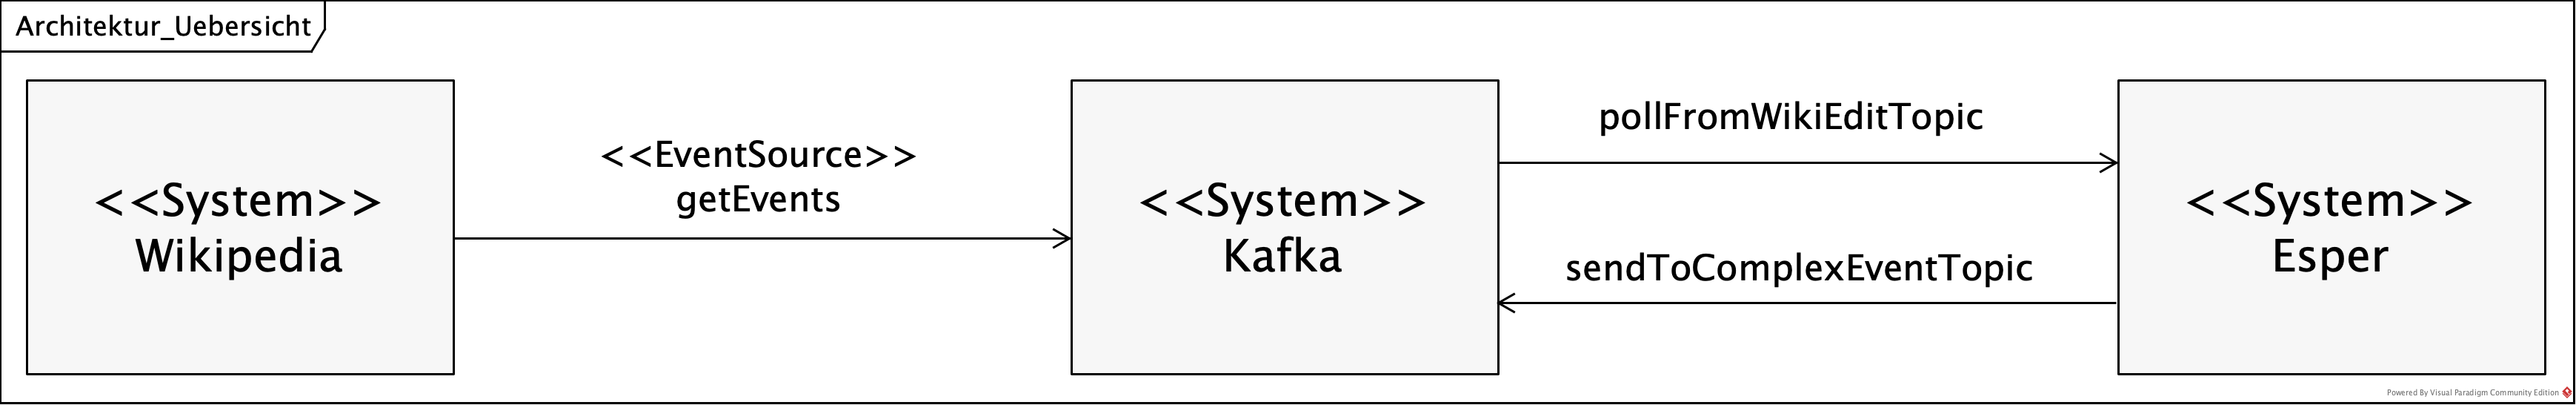
\includegraphics[width=.5\textwidth]{images/Architektur_Uebersicht.png}
    \caption{Architekturübersicht}
    \label{fig:architektur_uebersicht}
\end{figure}

Abbildung \ref{fig:architektur_uebersicht} zeigt bisher nur eine sehr rudimentäre Übersicht und soll als Grundlage dienen.
Die Verbindung zwischen Esper und Kafka muss noch genauer werden: Protokoll, senden von komplexen Events in neue Kafka-Topics.

\subsection{Collection Tier: Wikipedia}
\begin{itemize}
    \item Was für Daten nutzen wir? WikipediaEditEvents
    \item Welche konkreten Daten hat ein WikipediaEditEvent?
    \item Wie sieht das System dahinter aus; wie verarbeitet Wikipedia die Daten: Kafka
    \item Was ist EventSource und was bringt es hier?
\end{itemize}

\subsection{Implementierungsdetails zum Messaging queuing tier: Kafka}
Im Messaging Queuing Tier setzen wir Apache Kafka in der Version 2.1 ein, um die Wikipedia-Events aus dem Collection Tier
in unser eigenes Messaging-System zu überführen. In der Java-Anwendung werden die folgenden
Schritte nacheinander ausgeführt:
\begin{enumerate}
    \item \textit{Kafka Initialisierung.} Den Host des Bootstrap-Servers setzen. Als Key- und Value-Serialisierer setzen wir
    jeweils den \code{StringSerializer} von Kafka ein. Das heißt, die Events werden als JSON-String in das Topic \code{wikiEdit}
    eingespeist. Zum Senden von Events erzeugen wir ein Producer-Objekt mit dem passenden Typ \code{Producer<String, String>}.
    TODO: Vor- und Nachteile für eine De-/Serialisierung von der eigenen WikipediaEditEvent-Klasse diskutieren
    \item \textit{Erzeugung eines EventHandlers.} Für das Empfangen von EventSource-Nachrichten nutzen wir die Java-Bibliothek
    \textit{okhttp-eventsource}\footnote{https://github.com/launchdarkly/okhttp-eventsource}. Zur Verarbeitung der Events
    \code{onOpen}, \code{onClose}, \code{onMessage}, \code{onComment} und \code{onError} muss das Interface \code{EventHandler} von
    \textit{okhttp-eventsource} implementiert werden.
    \item \textit{Erzeugung und Starten einer EventSource.} Mit der Stream-URI der Wikipedia-EventSource und des implementierten EventHandler-Interfaces
    kann ein \code{EventSource}-Objekt erzeugt werden. Das Objekt dient dem Starten und Beenden eines EventSource-Streams.
    \item \textit{Beim Eintreffen eines Events, Senden einer Nachricht in ein Kafka-Topic.} Tritt ein Wikipedia-Event auf,
    wird die \code{onMessage}-Methode des implementierten EventHandlers-Interface aufgerufen. Einer der beiden Parameter enthält die Daten
    des aufgetretenen Events. Der Zugriff auf die als JSON-String codierte Nachricht erfolgt über die \code{getDate()}-Methode.
    Diese Daten sendet die Anwendung, über den zuvor erzeugten Producer, in das Kafka-Topic \code{wikiEdit}.
\end{enumerate}

TODO:
- Die Konfiguration von Kafka: Welche Topics gibt es? Partitionen? Consumer Groups? Replication? Persistence? (oder alles schon im vorherigen Kapitel schreiben)
- Vor- und Nachteile für eine De-/Serialisierung von der eigenen WikipediaEditEvent-Klasse diskutieren und der Einsatz von GSON?

\subsection{Implementierungsdetails zum Analysis tier: Esper}
In unserer Esper-Anwendung, die Teil des Analysis Tier ist, nutzen wir Esper in Version 7.1 als Complex Event Processing-Werkzeug. Zur Verarbeitung
der Wikipedia-Events implementieren wir die folgenden Schritte:

Genaueres zu den erzeugten Expressions im nächsten Kapitel.

\begin{enumerate}
    \item \textit{Esper Initialisierung.} Die Initialisierung von Esper besteht
    \item \textit{Expression erzeugen.}
    \item \textit{\code{UpdateListener} implementieren.}
    \item \textit{Kafka initialisieren.}
    \item \textit{Kafka Consumer erzeugen und in Endlosschleife Events pollen.}
    \item \textit{Empfangene Events auswerten.}
\end{enumerate}